\section{Response functions}

\subsection{Time definition}\label{subsec:time_definition}

A key concept in the analysis of the response functions is the time. Due to the
nature of the data, they are several options to define it.

In general, the time series are indexed in calendar time (hours, minutes,
seconds, milliseconds). Moreover, tick-by-tick data available on financial
markets all over the world is time stamped up to the millisecond, but the order
of magnitude of the guaranteed precision is much larger, usually one second or
a few hundreds of milliseconds \cite{empirical_facts,market_digest}. In several papers are
used different time definitions (calendar time, physical time, event time,
trade time, tick time) \cite{empirical_facts,sampling_returns,market_making}.
The TAQ data used in the analysis has the characteristic that the trades and
quotes can not be directly related due to the time stamp resolution of only one
second \cite{Wang_2016_cross}. Hence, it is impossible to match each trade with
the directly preceding quote. However, using a classification for the trade
signs, we can compute trade signs in two scales: trade time scale and physical
time scale.

The trade time scale is increased by one unit each time a transaction happens.
The advantage of this count is that limit orders far away in the order book do
not increase the time by one unit. The main outcome of trade time scale is its
``smoothing" of data and the aggregational normality \cite{empirical_facts}.

The physical time scale is increased by one unit each time a second passes.
This means that computing the responses in this scale involves sampling
\cite{sampling_returns,Wang_2016_cross}, which has to be done carefully when
dealing for example with several stocks with different liquidity. This sampling
is made in the trade signs and in the midpoint prices.

Facing the impossibility to relate midpoint prices and trade signs with the TAQ
data in trade time scale, we will use the midpoint price of the previous second
with all the trade signs of the current second. This will be our definition of
trade time scale analysis for the response function analysis.

For physical time scale, as we can sampling, we relate the unique value of
midpoint price of a previous second with the unique trade sign value of the
current second.

Thus, trade sign values will be used in trade time scale and physical time
scale and returns will be only used in physical time scale.

%%%%%%%%%%%%%%%%%%%%%%%%%%%%%%%%%%%%%%%%%%%%%%%%%%%%%%%%%%%%%%%%%%%%%%%%%%%%%%%
\subsubsection{Trade time scale}\label{subsubsec:trade_time}

We use the trade sign classification in trade time scale proposed by S. Wang et
al. in \cite{Wang_2016_cross} and used in
\cite{Wang_2017,Wang_2018_copulas,Wang_2016_avg} that reads

\begin{equation}\label{eq:trade_signs_trade}
    \varepsilon^{t}\left(t,n\right)=\left\{
    \begin{array}{cc}
    \text{sgn}\left(S\left(t,n\right)-S\left(t,n-1\right)\right),
    & \text{if }\\ S\left(t,n\right) \ne S\left(t,n-1\right)\\
    \varepsilon\left(t,n-1\right),
    & \text{otherwise}
    \end{array}\right.
\end{equation}

$\varepsilon^{t}\left( t,n \right) = +1$ implies a trade triggered by a market
order to buy, and a value $\varepsilon^{t}\left( t,n \right) = -1$ indicates a
trade triggered by a market order to sell.

In the second case of the classification, if two consecutive trades with the
same trading direction did not exhaust all the available volume at the best
quote, the trades would have the same price, and in consequence they will have
the same trade sign.

With this classification we obtain trade signs for every single trade in the
data set. According to \cite{Wang_2016_cross}, the average accuracy of the
classification is $85\%$ for the trade time scale.

TAQ time step is one second, and as it is impossible to find the
correspondences between trades and midpoint prices values inside a second step,
We used the last midpoint price of every second as the representative value of
each second. This introduce an apparent shift between trade signs and returns.
In fact, we set the last midpoint price from the previous second as the first
midpoint price of the current second, as explained in \cite{Wang_2016_cross}.

As we know the second in which the trades were made, we can relate the trade
signs and the midpoint prices as shown in Fig.
\ref{fig:relation_trades_midpoint_trade_scale}. For the trade time scale, they
are in general, several midpoint prices in a second. For each second we
select the last midpoint price value, and we relate it to the next second
trades. In Fig. \ref{fig:relation_trades_midpoint_trade_scale}, the last
midpoint price (circle) between the second $-1$ and $0$ is related with all the
trades (squares and triangles) in the second $0$ to $1$, and so on. It is worth
to note, in the seconds that there are no changes in the quotes, it is used the
value of the previous second (vertical line over the physical time interval).
Thus, all the seconds in the open market time have a midpoint price value, and
in consequence returns values. We assume that as long as they were not changes
in the quotes, the midpoint price remain the same as the one of the previous
second.

\begin{figure}[htbp]
    \centering
    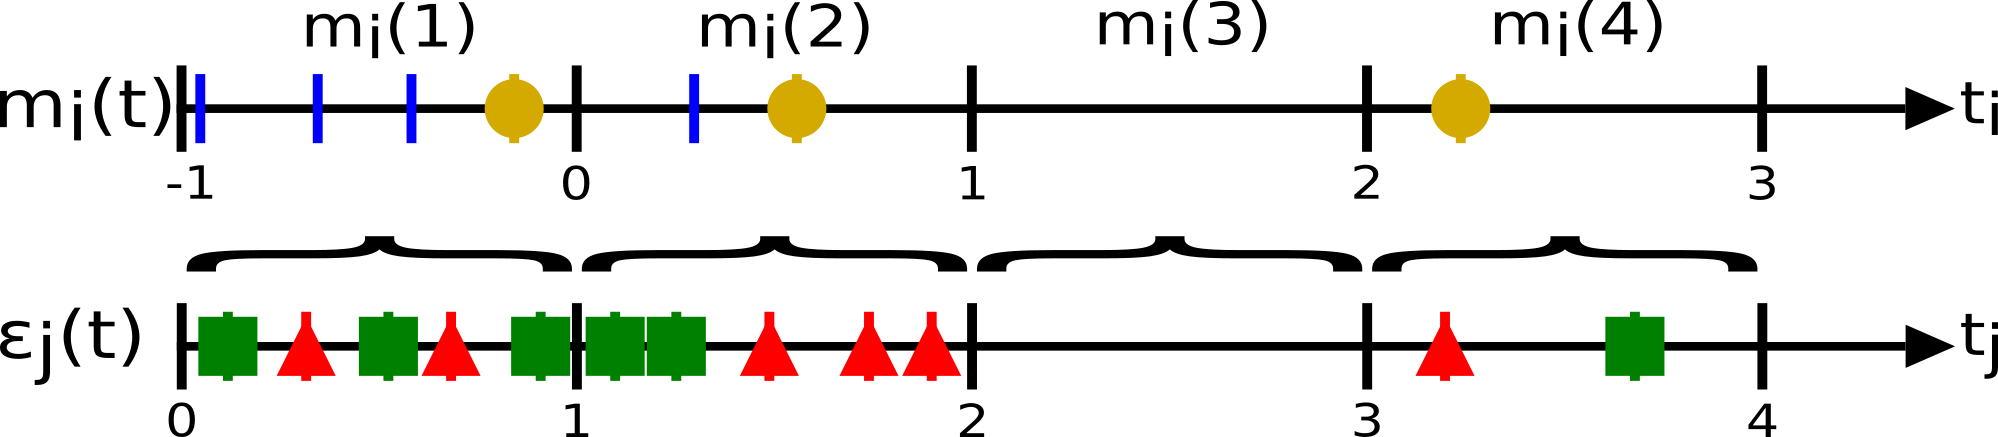
\includegraphics[width=\columnwidth]
    {figures/02_relation_trades_quotes_trade_scale.png}
    \caption{Sketch of data processing for trade time scale. In the midpoint
             price time line, the vertical lines represent the change in price
             of the quotes and the circles represent the last price change in a
             quote in a second. In the trade signs time line, the squares
             represent the buy market orders and the triangles represent the
             sell market orders. The midpoint price time line and the trade
             sign time line are shifted in one second.}
    \label{fig:relation_trades_midpoint_trade_scale}
\end{figure}

We computed all the analysis for the trade time scale using Equations
\ref{eq:midpoint_price_return} and \ref{eq:trade_signs_trade}.

The methodology described is an approximation to compute the response in the
trade time scale. A drawback in the computation could come from the fact that
the return of a given second is composed by the contribution of small returns
corresponding to each change in the midpoint price during a second. As we are
assuming only one value for the returns in each second, we are supposing  all
the returns in one second interval to be positive or negative with the same
magnitude, which could not be the case. This could increase or decrease the
response signal at the end of the computation.

\begin{figure}[htbp]
    \centering
    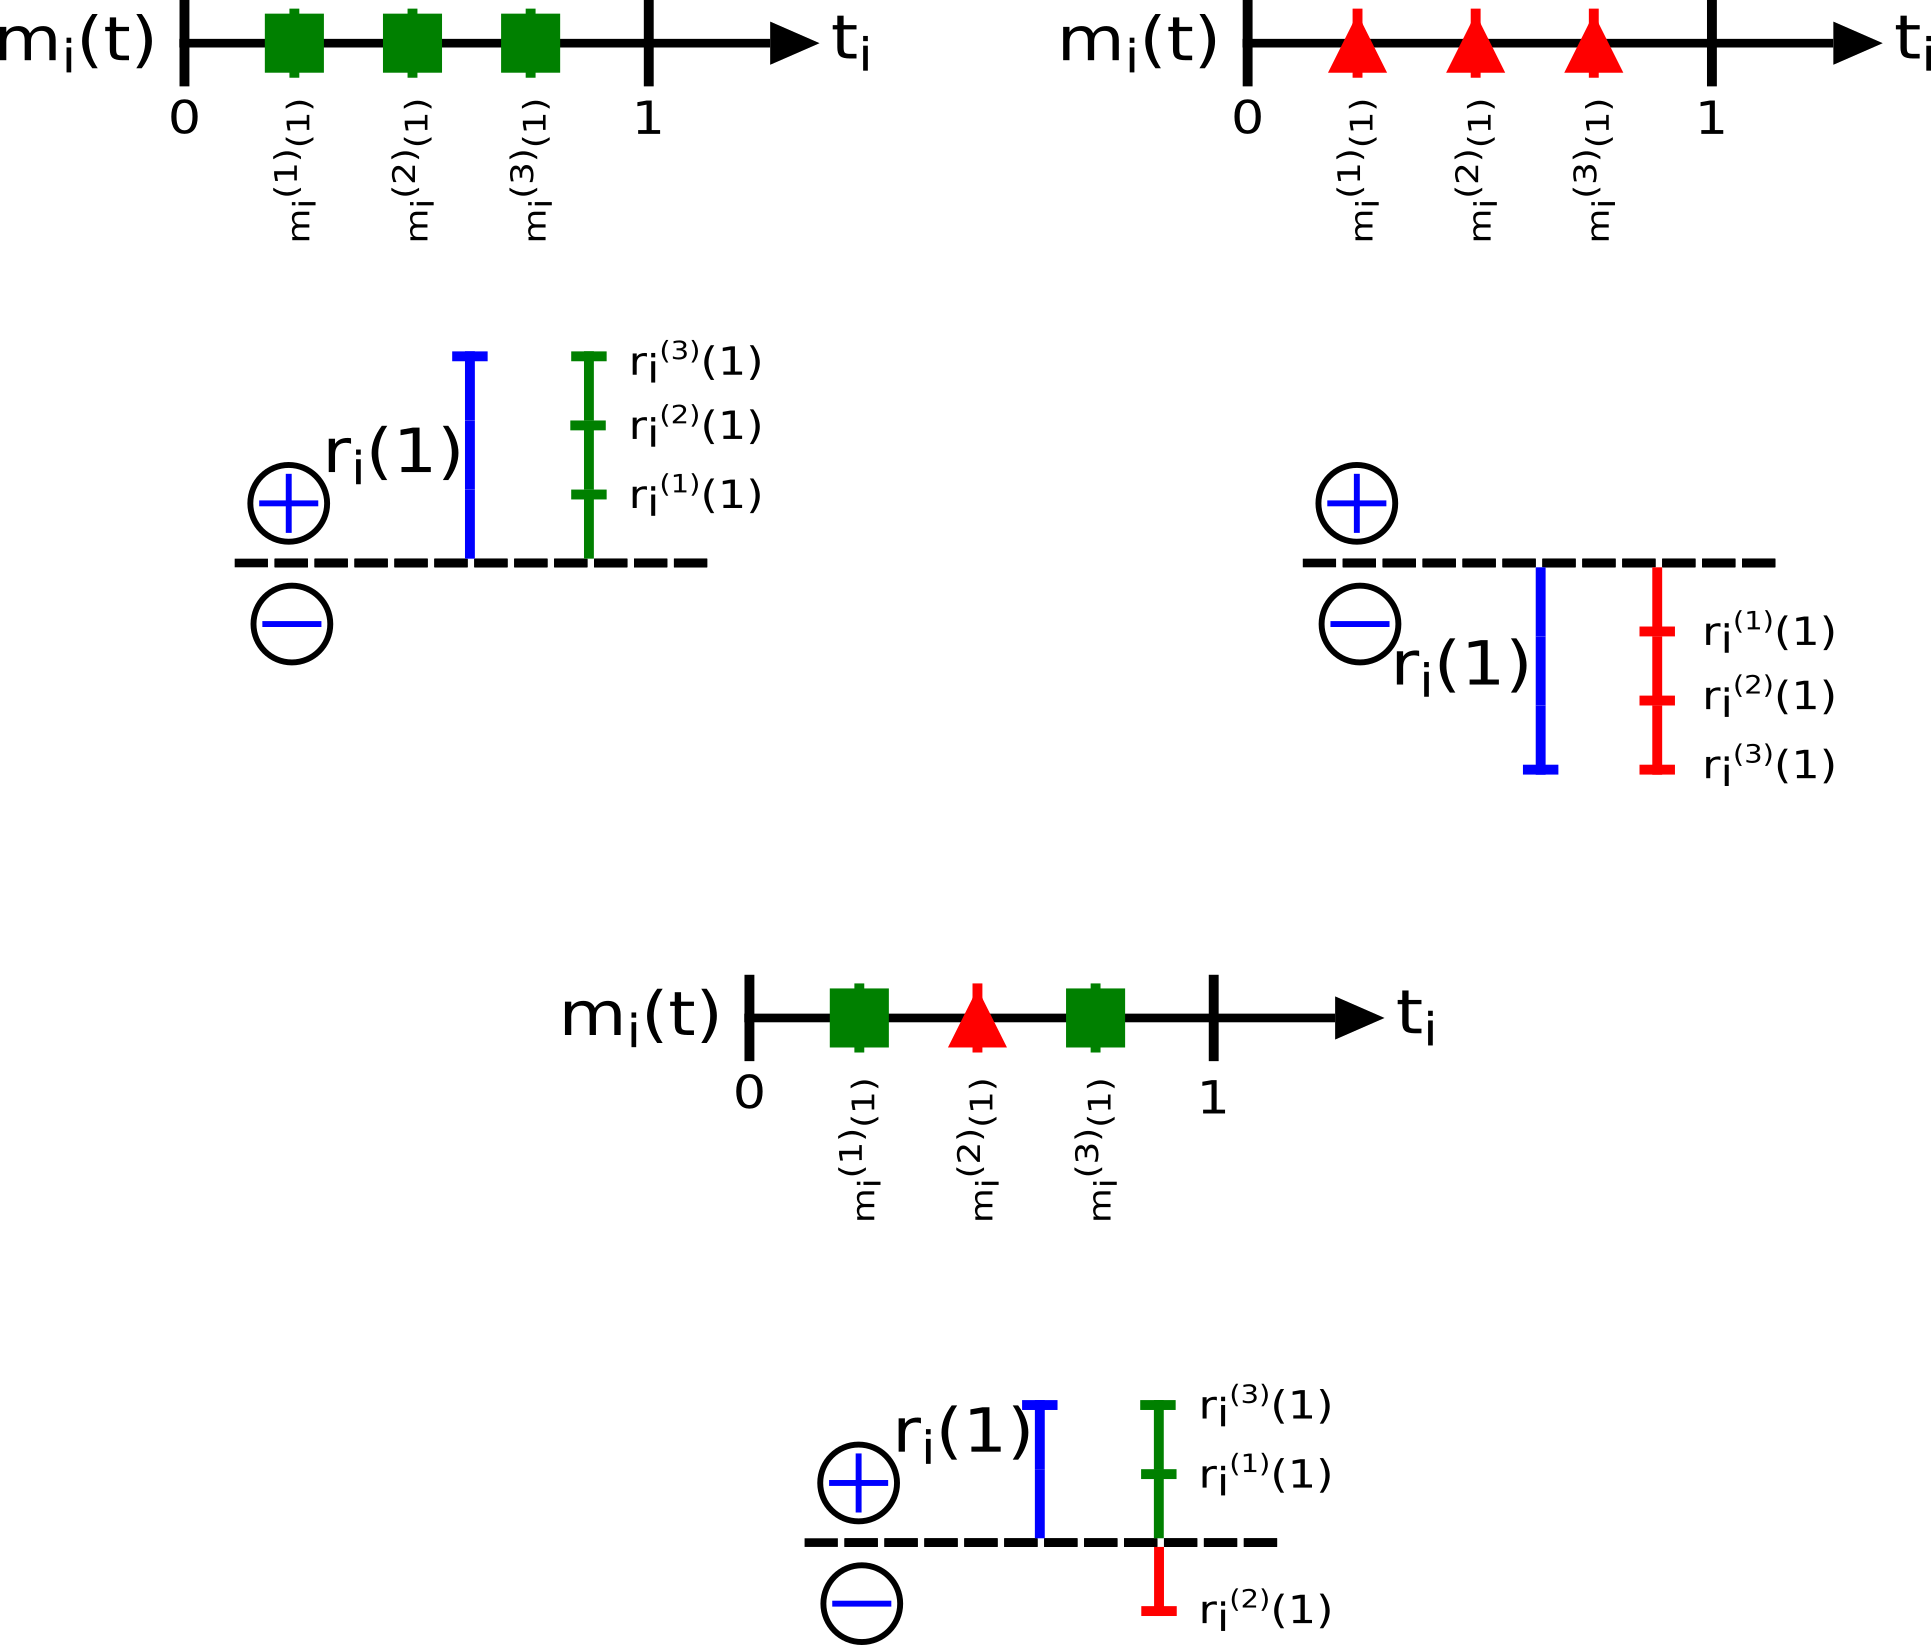
\includegraphics[width=\columnwidth]{figures/02_return_contributions.png}
    \caption{Sketch of the return contributions from every midpoint price
             change in a second. The squares represent the rise of the price of
             the midpoint price and the triangles represent the decrease of the
             price of the midpoint price. We illustrate three cases: (top left)
             the changes of the midpoint prices and return are due to the rise
             of the prices, (top right) the changes of the midpoint prices and
             return are due to the decrease of the prices, and (bottom) the
             changes of the midpoint prices and return are due to a combination
             of rise and decrease of the prices.}
    \label{fig:return_contributions}
\end{figure}

Figure \ref{fig:return_contributions} illustrate with one example this point.
Suppose one second interval, in which they are three different midpoint prices,
and as result, three different returns for this three midpoint price
values. Furthermore, consider that the volume of limit orders that have the
corresponding midpoint prices are the same in the bid and in the ask (so the
returns have the same magnitude). In the case of the top left (top right)
sketch, all the changes are due to the rise (decrease) of the midpoint price,
that means, consumption of the best ask (bid), so all the contributions of the
individual returns in the second are positive (negative), and in consequence,
the net return is positive (negative). In the case of the bottom, the changes
are due to a combination of increase and decrease of the midpoint price, so in
the end the individual returns sum up to a net return, which can be positive or
negative, depending of the type of midpoint price values in the interval. Thus,
in this case, we are assuming at the end that all the returns were positive or
negative, what probably was not the case, and in consequence will increase or
decrease the real value of the net return.

In all the cases we choose the last change in the midpoint price in a second
interval as described before
(Fig. \ref{fig:relation_trades_midpoint_trade_scale}). We use this method
knowing that the variation in one second of the midpoint price is not large
(in average, the last midpoint price of a second differ with the average
midpoint of that second in $0.007\%$), so it can give us valuable information
about the response functions.

%%%%%%%%%%%%%%%%%%%%%%%%%%%%%%%%%%%%%%%%%%%%%%%%%%%%%%%%%%%%%%%%%%%%%%%%%%%%%%%
\subsubsection{Physical time scale}\label{subsubsec:physical_time}

We use the trade sign definition in physical time scale proposed by
S. Wang et al. in \cite{Wang_2016_cross} and used in
\cite{Wang_2017,Wang_2016_avg}, that depends on the classification in
Eq. \ref{eq:trade_signs_trade} and reads

\begin{equation}\label{eq:trade_signs_physical}
    \varepsilon^{p}\left(t\right)=\left\{
    \begin{array}{cc}
    \text{sgn}\left(\sum_{n=1}^{N\left(t\right)}\varepsilon^{t}
    \left(t,n\right)\right),
    & \text{If }N \left(t\right)>0\\
    0, & \text{If }N\left(t\right)=0
    \end{array}\right.
\end{equation}

Where $N \left(t \right)$ is the number of trades in a second interval.
$\varepsilon^{p}\left( t \right) = +1$ implies that the majority of
trades in second $t$ were triggered by a market order to buy, and a value
$\varepsilon^{p}\left( t \right) = -1$ indicates a majority of sell
market orders. In this definition, they are two ways to obtain
$\varepsilon^{p}\left( t \right) = 0$. One way is that in a particular
second there is not trades, and then no trade sign. The other  way is that the
addition of the trade signs ($+1$ and $-1$) in a second be equal to zero. In
this case, there is a balance of buy and sell market orders.

Market orders show opposite trade directions to limit order executed
simultaneously. An executed sell limit order corresponds to a buyer-initiated
market order. An executed buy limit order corresponds to a seller-initiated
market order.

As in the trade time scale, in the physical time scale we use the same strategy
to obtain the midpoint price for every second, so all the seconds in the open
market time have a midpoint price value. It is worth to note again, that even
if the second does not have a change in quotes, it will has still a midpoint
price value and a return value.

\begin{figure}[htbp]
    \centering
    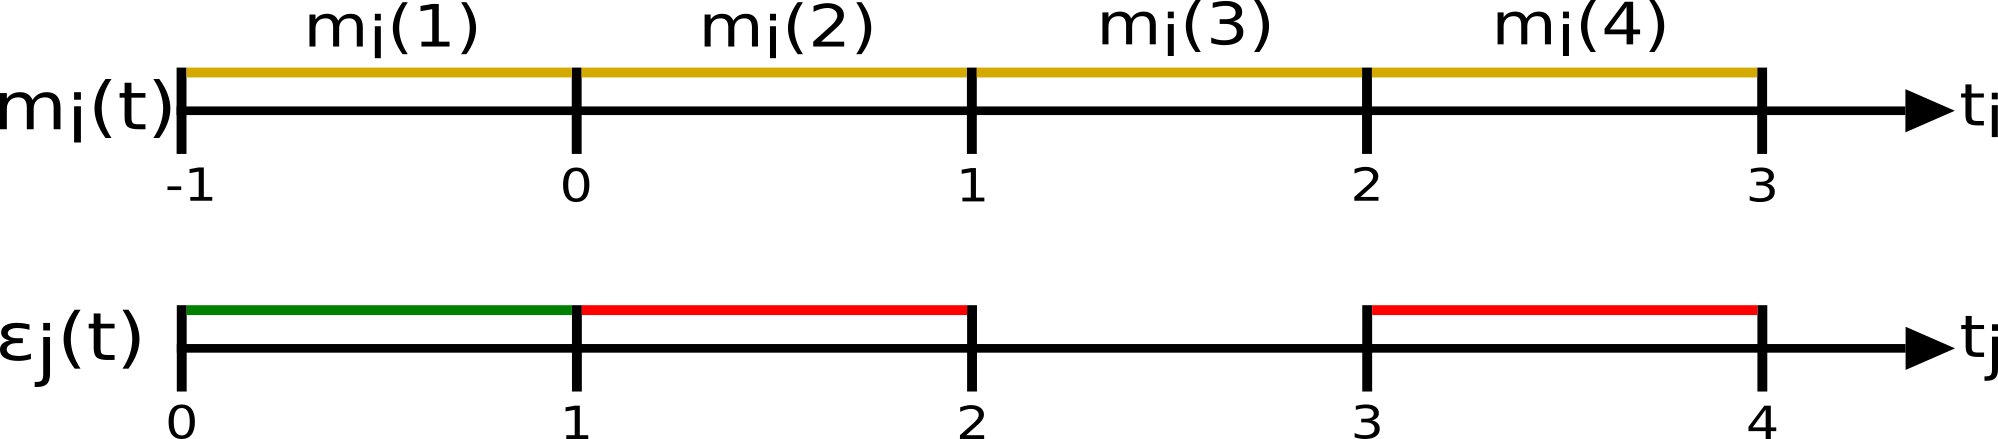
\includegraphics[width=\columnwidth]
    {figures/02_relation_trades_quotes_time_scale.png}
    \caption{Sketch of data processing for physical time scale. In the midpoint
             price time line, the horizontal lines between seconds represent
             the midpoint prices. In the trade signs time line, the horizontal
             lines between seconds represent the trade sign values. The
             midpoint price time line and the trade sign time line are shifted
             in one second.}
    \label{fig:relation_trades_midpoint_time_scale}
\end{figure}

In this case we do not compare every single trade sign in a second, but the net
trade sign obtained for every second with the definition. This can be seen in
Fig. \ref{fig:relation_trades_midpoint_time_scale}, we related the midpoint
price of the previous second with the trade sign of the current second.

According to \cite{Wang_2016_cross}, this definition has an average
accuracy up to $82\%$ in the physical time scale.

%%%%%%%%%%%%%%%%%%%%%%%%%%%%%%%%%%%%%%%%%%%%%%%%%%%%%%%%%%%%%%%%%%%%%%%%%%%%%%%

The average of the best ask and the best bid is the midpoint price, which is
defined as \cite{subtle_nature,Bouchaud_2004,large_prices_changes,prop_order_book}

\begin{equation}\label{eq:midpoint_price}
    m\left(t\right)=\frac{a\left(t\right)+b\left(t\right)}{2}
\end{equation}

As the midpoint price depends on the quotes, it changes if the quotes change.
The midpoint price grows if the best ask or the best bid grow. This happen if
someone buys and consumes all the volume of the sell limit order with the price
of the best ask, or someone sets a buy limit order with a bigger price than the
previous best bid, or there is a cancellation of the best ask.

On the other hand, the midpoint price decreases if the best ask or the best bid
decrease. This happen if someone sells and consumes all the volume of the buy
limit order with the price of the best bid, or someone sets a sell limit order
with a lower price than the previous best bid, or there is a cancellation of
the best bid.

The midpoint price will not change if there is no activity in the market.

Price changes are typically characterized as returns. If one denotes
$S\left( t\right)$ the price of an asset at time $t$, the return
$r\left(t\right)$, at time $t$ and time lag $\tau$ is simply the relative
variation of the price from $t$ to $t + \tau$
\cite{subtle_nature,empirical_facts,asynchrony_effects_corr,tick_size_impact,causes_epps_effect,non_stationarity},

\begin{equation}\label{eq:return_general}
    r^{g} \left(t, \tau \right) = \frac{S\left(t + \tau\right)
    - S\left(t\right)}{S\left(t\right)}
\end{equation}

It is also common to define the returns as
\cite{dissecting_cross,subtle_nature,empirical_facts,empirical_properties,large_prices_changes,theory_market_impact,spread_changes_affect,fluctions_market_friction,pow_law_dist,rand_mat}

\begin{equation}\label{eq:log_return_general}
    r^{l}\left(t,\tau\right) = \ln S\left(t + \tau\right)
    - \ln S\left(t\right) = \ln \frac{S\left(t + \tau\right)}{S\left(t\right)}
\end{equation}

Equation \ref{eq:return_general} and Eq. \ref{eq:log_return_general} coincide
if $\tau$ is small enough \cite{subtle_nature,empirical_facts}.

At longer timescales, midpoint prices and transaction prices rarely differ by
more than half the spread. The midpoint price is more convenient to study
because it avoids problems associated with the tendency of transaction prices
to bounce back and forth between the best bid and ask
\cite{large_prices_changes}.

We define the returns via the midpoint price as

\begin{equation}\label{eq:midpoint_price_return}
    r\left(t,\tau\right) = \frac{m\left(t+\tau\right)-m\left(t\right)}
    {m\left(t\right)}
\end{equation}

The distribution of returns is strongly non-Gaussian and its shape continuously
depends on the return period $\tau$. Small $\tau$ values have fat tails return
distributions \cite{subtle_nature}.

Then we can expect three kind of values of the returns. The returns are
positive values, when the midpoint price
$m\left(t+\tau\right) > m\left(t\right)$, hence, there is a buy in the market
or there is a cancellation of the best ask or an addition in the best bid
during the time lag $\tau$. The returns are negative values, when the midpoint
price $m\left(t+\tau\right) < m\left(t\right)$, thus, there is a sell in the
market, or there is a cancellation of the best bid or an addition in the best
ask during the time lag $\tau$. The returns are zero when there is no activity
during the time lag $\tau$.

The trade signs are defined for general cases as

\begin{equation}\label{eq:trade_sign_general}
    \varepsilon\left(t\right)=\text{sign}\left(S\left(t\right)
    -m\left(t-\delta\right)\right)
\end{equation}

where $\delta$ is a positive time increment. Hence we have

\begin{equation}\label{eq:trade_sign_results}
    \varepsilon\left(t\right)=\left\{
    \begin{array}{cc}
    +1, & \text{If } S\left(t\right)
    \text{ is higher than the last } m\left( t \right)\\
    -1, & \text{If } S\left(t\right)
    \text{ is lower than the last } m\left( t \right)
    \end{array}\right.
\end{equation}

$\varepsilon(t) = +1$ indicates that the trade was triggered by a market order
to buy and a trade triggered by a market order to sell yields
$\varepsilon(t) = -1$
\cite{subtle_nature,Bouchaud_2004,spread_changes_affect,quant_stock_price_response,order_flow_persistent}.

It is well-known that the series of the trade signs on a given stock exhibit
large autocorrelation. A very plausible explanation of this phenomenon relies
on the execution strategies of some major brokers on given markets. These
brokers have large transactions to execute on the account of some clients. In
order to avoid market making move because of an inconsiderable large order,
they tend to split large orders into small ones \cite{empirical_facts}.

INCLUDE response function from \cite{prop_order_book}

The response function is used to study the mutual dependence between stocks. In
\cite{r_walks_liquidity,Bouchaud_2004}, Bouchaud et al. use the response
function that only depends on the time lag $\tau$

\begin{equation}\label{eq:Bouchaud_2004}
    R\left(\tau\right)=\left\langle \left(S_{n+\tau}-S_{n}\right) \cdot
    \varepsilon_{n}\right\rangle_{trades}
\end{equation}

Where $\varepsilon_{n}$ is the sign of the $n^{th}$ trade and the price $S_n$
is defined as the midpoint just before the $n^{th}$ trade
($S_{n} \equiv m_{n^{-}}$).
The quantity $R\left(\tau\right)$ measures how much, on average, the price
moves up (down) at time $\tau$ conditioned to a buy (sell) order at time zero.

In a later work \cite{Wang_2016_cross}, S. Wang et al. use the logarithmic
return for stock $i$ and time lag $\tau$, defined via the midpoint price
$m_{i} \left( t \right)$. The cross-response function is then defined as

\begin{equation}\label{eq:Wang_2016}
    R_{ij}\left(\tau\right)=\left\langle r_{i}\left(t-1,\tau\right)\cdot
    \varepsilon_{j} \left(t\right) \right\rangle _{t}
\end{equation}

Finally, in \cite{Wang_2018_b}, S. Wang et al. define the response function as

\begin{equation}\label{eq:Wang_2018_b}
    R_{ij} = \left\langle \left(\ln m_{i}^{\left(f\right)}\left(t_{j}\right)-
    \ln m_{i}^{\left(p\right)} \left(t_{j}\right) \right)\cdot\varepsilon_{j}
    \left(t_{j}\right)\right\rangle _{t_{j}}
\end{equation}

For the price change of stock $i$ caused by a trade of stock $j$.

Here, $m_{i}^{\left(p\right)}\left(t_{j}\right)$ is the midpoint price of stock
$i$ previous to the trade of stock $j$ at its event time $t_j$ and
$m_{i}^{\left(f\right)}\left(t_{j}\right)$ is the midpoint price of stock $i$
following that trade.
